\section{Merging Heuristics}
\indent Unfortunately, although the label-swapping algorithm yields perfectly satisfying graphs, it often doesn't sufficiently disguise a given graph.  In this section, we present a heuristic, called \emph{adjacency group merges} (or simply \emph{merges}) that further randomizes a given graph, but is not guaranteed to maintain the same k-neighborhood.

\begin{definition}
\noindent A \emph{merging} of a graph's adjacency groups combines similar adjacency groups into larger groups containing the union of their nodes based on their \emph{difference}. The difference between adjacency groups $A$ and $B$ is the size of the symmetric difference of $N_k(v)$ and $N_k(u)$, for $v \in A$ and $u \in B$. 
\end{definition}

\subsection{Non-Deterministic Merging}

%\indent This process takes in two values \emph{maximum difference} and %\emph{}

\begin{figure}[ht]
  \label{merge_k_2}
  \centering
  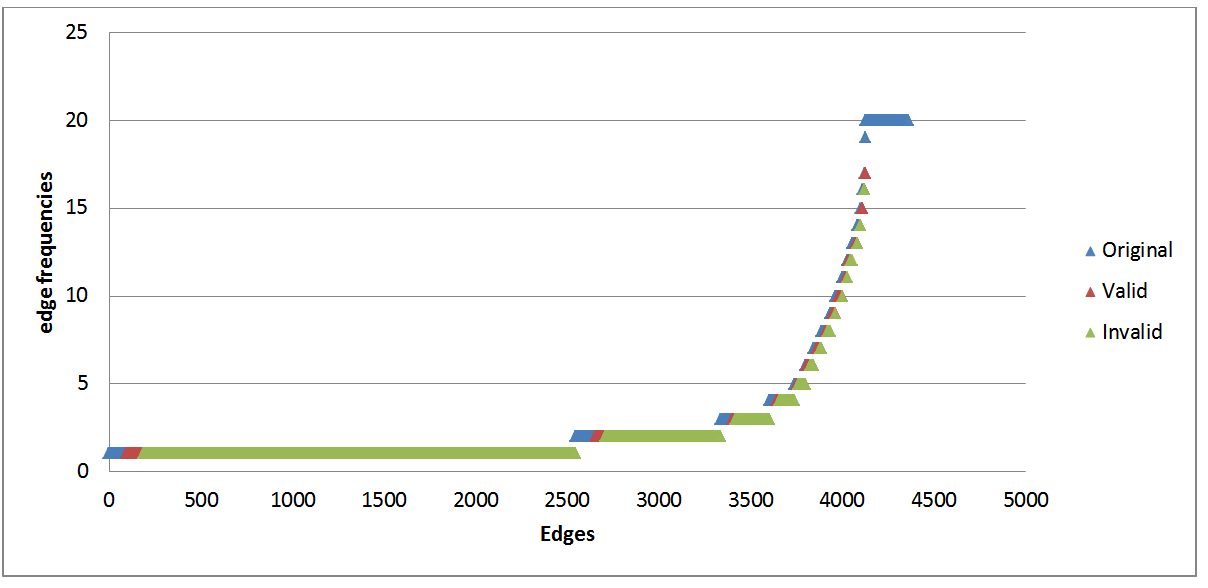
\includegraphics[scale=0.4]{mu=0_1 k=2 non-det merge 5.png}
  \caption{The results of the non-deterministics merging where mu=0.1 and k=2}
  \label{fig:merge_k_2}
\end{figure}

\begin{figure}[htb]
  \label{merge_k_5}
  \centering
  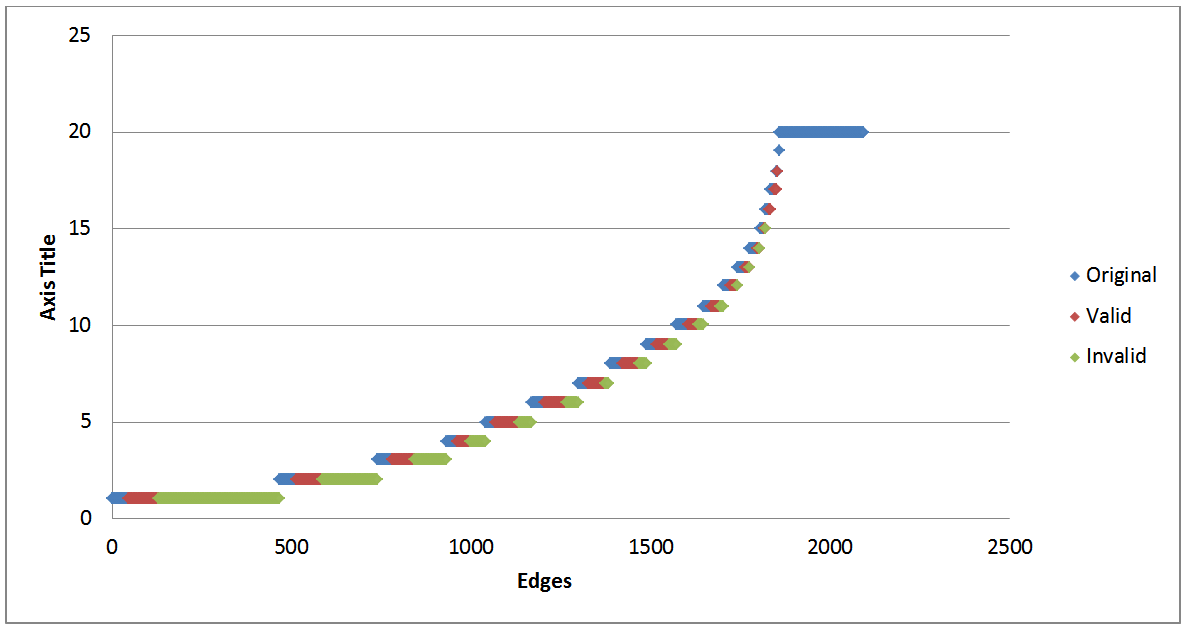
\includegraphics[scale=0.4]{mu=0_1 k=5 non-det merge 5.png}
  \caption{The results of the non-deterministics merging where mu=0.1 and k=5}
  \label{fig:merge_k_5}
\end{figure}

\begin{definition}
An \emph{adjacency group merging} maps every pair of nodes to  the differencence value between their adjacency groups and merges adjacency groups of the first n that have not been involved in a previous merge.
\end{definition}

\begin{center}
	\begin{tabular}{l}
    	{\bf input:} graph $G=(V,E)$, k-neighborhoods $K= \{k_{1}, k_{2}, ...\}$, \\
        \hspace{12 mm} adjecency groups $A=\{a_{1}, a_{2}, ...\}$, limit L \\
        {\bf output:} adjecency groups A* \\
        for all $v \in V$: \\
        \hspace{5 mm} for all $w \in V$ where $v \neq w$: \\
        \hspace{10 mm} find $Diff(A(v), A(w))$ \\
        \hspace{5 mm} end \\
        end \\
        $n = 0$
        for all $(v,w,d) \in V \times V \times \mathbb{Z}$ sorted by $d=Diff(A(v), A(w))$ where $v \neq w$: \\
        \hspace{5 mm} if $not\_merged(A(v))$ and $not\_merged(A(w))$:  \\
        \hspace{10 mm} $merge(A(v),A(w))$ \\
        \hspace{10 mm} $mark\_as\_merged(A(v))$ \\
        \hspace{10 mm} $mark\_as\_merged(A(w))$ \\
        \hspace{10 mm} $n++$ \\
        \hspace{10 mm} if $n == L$: \\
        \hspace{15 mm} break \\
    \end{tabular}
\end{center}